\documentclass[sigconf]{acmart}
\AtBeginDocument{%
  \providecommand\BibTeX{{%
    \normalfont B\kern-0.5em{\scshape i\kern-0.25em b}\kern-0.8em\TeX}}}
\setcopyright{rightsretained}
\acmConference[SNACS '22]{Social Network Analysis for Computer Scientists Course 2022}{Master CS, Fall 2022}{Leiden, the Netherlands}
\copyrightyear{2022}
\acmYear{2022}
\acmISBN{}
\acmDOI{}
%%%% Do not modify lines 1-11

\usepackage{subcaption}

\begin{document}

\title{node2vec Based Graph Convolutional Networks}
\subtitle{ Social Network Analysis for Computer Scientists --- Course paper} % do not modify this

\author{Chenyu Shi}
\email{s3500063@umail.leidenuniv.nl}
\affiliation{
  \institution{LIACS, Leiden University}
  \city{Leiden}
  \country{Netherlands}}

\author{Shupei Li}
\email{s3430863@umail.leidenuniv.nl}
\affiliation{
  \institution{LIACS, Leiden University}
  \city{Leiden}  
  \country{Netherlands}}

\renewcommand{\shortauthors}{Shi and Li}

\keywords{node2vec, GCN, graph embeddings, social network analysis, network science}

\begin{abstract}

% the abstract summarizes the entire paper: context, problem, solution, approach, data, experimental results, conclusion and real-world implications. but, shortly, so in half a column or so.

\end{abstract}

\maketitle

\section{Introduction}
% textual description of the context, the problem considered, why it is important, how it is addressed in other works, and what real-world applications are. end with a paragraph on what the contributions of the paper are (so, which problems you solve or which research questions you address), and finally a paragraph on how the remainder of the paper is organized.
Graphs are mathematical objects that can model complex relationships on non-Eucildean space. They are widely used in multiple domains such as molecular structure modelling, social network analysis, recommender systems, etc. To leverage the information contained in graphs, it is essential to develop efficient techniques for representing graph-structured data numerically.\par
Traditional statistical and machine learning methods are designed for extracting features from structured data on Eucildean space. For example, principal component analysis(PCA), uniform manifold approximation and projection (UMAP), and t-distributed stochastic neighbor embedding (T-SNE) are common techniques to reduce dimensions and capture features of data. Although these methods have achieved satisfactory performance on structured-data, they are hard to be generalized to graph-structured data, because they highly depend on properties of Eucildean space.\par
This challenge led to the development of techniques specifically for graph-based representation. There are two main types of these techniques: shallow embedding method and deep embedding method \cite{murphy2022}. Shallow embedding methods use shallow encoder functions to map the original graph structure onto a Euclidean space and obtain the embedding matrix. If data is labelled, we can apply supervised learning algorithms, e.g. label propagation, to extract embeddings later used in a supervised task. However, labels are not available or only partly available in most cases, where we need unsupervised learning or semi-supervised learning to distill information about graph structure. These methods can be divided into distance-based method and outer product method further \cite{murphy2022}. Generally, distance-based methods select a metric function that indicates distances between any pairs of nodes and optimize the function to generate embeddings. Representative distance-based methods include multi-dimensional scaling and laplacian eigenmaps. Outer product-based methods use matrix operations to evaluate the similarity between nodes. Most of early studies in graph embedding field adopt matrix factorization to reduce dimensionality of data while preserve the structure information \cite{cai2018}. Another mainstream outer product-based method is inspired by the development in natural language processing. Existing research generalizes the skip-gram word embedding framework to capture the graph embeddings, which has been proved to be efficient on many graph related tasks \cite{deepwalk}\cite{line}. Node2vec \cite{node2vec}, one of algorithms addressed in this paper, is also a variation of skip-gram-based method.\par
Node2vec is a semi-supervised algorithm whose goal is learning features from networks \cite{node2vec}. It transforms the graph embedding learning into a maximum likelihood optimization problem in a similar way to skip-gram architecture of word embedding learning. Likelihood calculation requires a clear definition of the neighborhood. Textual data has the intrinsic semantic order that can be naturally employed as word neighborhoods. However, graph-structured data has no explicit neighborhoods. Node2vec introduces the idea of the second-order random walk into graph neighborhood sampling strategy. The emphasis of node2vec model is easy to switch between breadth-first sampling (BFS) and depth-first sampling (DFS) by adjusting hyperparameters. Moreover, its computational complexity is less than classical BFS and DFS strategies. Because of its efficiency and great performance on graph embedding learning task, node2vec is an ideal choice among shallow embedding methods.\par
In recent years, a lot of studies have focused more on deep embedding method rather than the shallow one. Deep embedding method usually refers to algorithms that learn graph features via graph neural networks (GNN). The GNN is a class of artificial neural networks constructed for graph-structured data. Inspired by the success of convolutional neural networks (CNN) on grid data, many GNN architectures have been proposed to generalize the convolution operation on graphs. In this paper, we mainly focus on a method called graph convolutional networks (GCN) \cite{gcn}. GCNs defines the graph convolution based on the graph Laplacian spectrum. It has achieved state-of-the-art performance on common graph related tasks, such as node classification, link prediction, etc.\par
We propose a novel method to extract embeddings from graphs in this paper. Our method is based on node2vec and GCNs. Motivated by the concept of meta learning, we regard the embeddings returned by node2vec as the meta information for GCNs. This prior knowledge helps to improve the quality of final graph embeddings, and therefore enhances the model performance in various tasks.\par
The rest of the paper is organized as follows. Section 2 reviews related works on graph embedding learning methods. We illustrate basic task notations and framework in Section 3. And then we describe approaches in detail in Section 4. Section 5 is an introduction to five open source data sets we use in the project. After that, we present our experimental set-up and results in Section 6. The paper ends with a conclusion section.  

\section{Related work}
% briefly discuss other papers related to this work, or previous work describing other approaches for the same problem. end with a statement on how your paper contributes to these works.
Our project draws inspiration both from the skip-gram-based shallow embedding method and the deep embedding method. The following will briefly review existing works related to these methods.\par
Skip-gram-based methods optimize graph embeddings to predict nodes in the defined context. Actually, this kind of methods leverages the matrix factorization technique implicitly \cite{murphy2022}. Compared to early works that explicitly use matrix factorization, skip-gram-based methods are usually more computationally efficient. Deepwalk \cite{deepwalk}, an algorithm proposed in 2014, is one of pioneering studies that generalizes the idea of skip-gram model in language processing to graph embedding learning field. Deepwalk models the context of nodes by truncated random walks, which is analogous to sentences in textual data. It utilizes the local information obtained from random walks and learns a latent space that corresponds to features of vertices. Following the Deepwalk, LINE algorithm \cite{line} is proposed to address the preservation of network properties and applicability on large-scale networks. The neighborhood sampling strategy of LINE is firstly simulating a BFS-style search for half of the feature dimensions and then a DFS-style search for remaining dimensions. Both Deepwalk and LINE are restricted to a specific sampling strategy of neighborhoods. Node2vec \cite{node2vec} algorithm provides a more flexible option. It introduces a return parameter and an in-out parameter during second-order random walks that enables users to adjust the style of sampling. Its workflow is similar to Deepwalk and can be considered as a generalization.\par
GNNs have been extensively researched these years. Learning graph embeddings is one of the important applications of GNNs. According to \cite{murphy2022}, GNN models used to devise graph embeddings are called deep embedding methods. A main challenge in designing GNNs is finding an efficient and easy-to-train filter to process graph signals. One solution is applying graph Fourier transform to define the convolution operation on graphs. However, using a filter directly based on graph Laplacian matrix is computationally expensive. Defferrard et al. \cite{Defferrard2016} suggest to approximate the filter by the k-order Chebyshev polynomial, which has a practical computational complexity. Kipf and Welling \cite{gcn} propose GCN model that simplifies the approximation further. GCNs limit the order Chebyshev polynomial to one and assume the coefficients in polynomial are equal. Besides, GCNs consider the self-loops in the graph and intrduce the renormalization trick, which improves the quality of learned graph embeddings. So far, GCNs have achieved the great performance on different graph related tasks.\par
Based on these works, we make the following contributions in the project.
\begin{enumerate}
    \item We propose a novel method to learn graph embeddings, inspired by meta learning concept. Our method fully utilizes the information from node2vec and the power of GCN architecture. We test our model on node classification and link prediction task.
    \item We evaluate node2vec, GCN, and our proposed method on five real-word data sets. In node classification task, we use additional metrics to assess the model performance, i.e. accuracy, recall, and weighted f1-score, while the original paper of node2vec only reports macro f1-score.
\end{enumerate}



\section{Preliminaries}
\subsection{Feature Learning Framework}
Feature learning in networks is regarded as a a maximum likelihood optimization problem\cite{node2vec}. We represent the given network as $G=(V,E)$, where $V$ and $E$ are nodes set and edges set respectively. Feature Learning task aims to find a projection $f: V \rightarrow R^d$, such that $f$ optimizes the following objective function:
$$\mathop{max}\limits_{f} \sum_{u\in V}log\ Pr(N_s(u)|f(u))$$

Projection $f$ allocates each node an embedding vector with length $d$. In other words, projection $f$ can be formulated as a matrix of size $|V|\times d$. $N_s(u)\subset V$ defines \textit{network neighborhood} for a node $u$ with neighborhood sampling strategy $S$. Please be aware, this \textit{network neighborhood} is not equivalent to the commonly used concept \textit{local neighborhood} which only is determined by the graph structure. On the contrary, \textit{network neighborhood} is generated based on both network structure and sampling strategy. Therefore, the above formula aims to maximize the log-probability of observing a network neighborhood $N_s(u)$ for a node u conditioned on its feature embedding representation, given by projection $f$.

To simplify the above optimization formula and task, two standard assumptions are made. One is conditional independence, which means observing a neighborhood node is independent of observing any other neighborhood node. Then according to the property of independent event, the formula in the objective function above can be written in the form of multiplication:
$$Pr(N_s(u)|f(u))=\prod_{n_i\in N_s(u)}^N Pr(n_i|f(u))$$

The other is symmetry in feature space, which means each source node and its neighborhood node have a symmetric effect over each other in feature space. In the reference \cite{node2vec}, the conditional likelihood of each \textit{(source node, neighbor node)} pair in the network neighborhood is formulated as a softmax function:
$$Pr(n_i|f(u))=\frac{exp(f(n_i)\cdot f(u))}{\sum_{v\in V} exp(f(v)\cdot f(u))}$$

Finally, the objective function can be rewritten using the above two assumptions in the form of:
$$\mathop{max}\limits_{f} \sum_{u\in V}[-log\ \sum_{u\in V}exp(f(u)\cdot f(v))+ \sum_{n_i\in N_s(u)}f(n_i)\cdot f(u)]$$

The first half of this formula $-log\ \sum_{u\in V}exp(f(u)\cdot f(v))$ is very expensive in computing. Therefore, a negative sampling method is applied to calculate it approximately \cite{mikolov2013distributed}. For this objective function, stochastic gradient decent is applied to optimize it and obtain the projection $f$.

With a good designed network neighborhood sampling strategy $S$, the above optimization process could help to find projection $f$ which makes the nodes embedding equipped with homophily and structural equivalence information \cite{hoff2002latent}, which could be taken advantage of in the downstream task.

The sampling strategy $S$ is the most important part of feature learning framework. In this paper,  second order random walk, the key point of $Node2Vec$, is applied as the sampling strategy. Before we dive into the details of $Node2Vec$ and second order random walk in section 4.1, let us have a glance to two commonly used downstream tasks, nodes classification and link prediction, which can be used to measure the performance of the nodes embedding generated by $Node2Vec$. 

\subsection{Downstream Task}

Nodes embedding is widely used in many common tasks of networks, such as nodes classification and link prediction. These tasks, which take advantage of information from nodes embedding, are called downstream tasks. Therefore, the best way to examine whether the nodes embedding generated by Feature Learning Framework, such as $Node2Vec$, is to check the performance of nodes embedding on such downstream task.

In this paper, two downstream tasks are used.\par
\vspace{0.2cm}
\noindent\textbf{Nodes Classification}. Given a graph $G=(E,V)$ with category labels of part of nodes, nodes classification task aims to classify the rest of nodes without labels into their category correctly.\par
\vspace{0.2cm}
\noindent\textbf{Link prediction}. Given a subgraph $G'=(V',E)$ of the entire graph $G=(V,E)$, where $V'\subset V$ and the rest of edges are missing. Link prediction task aims to predict these missing edges correctly.\par
\vspace{0.2cm}
Nodes classification and link prediction are two basic but very important tasks in network analysis area. Therefore, it's of much importance to examine $Node2Vec$ whether works well in these two tasks.

The downstream tasks also need a model, such as a classifier like Logistic Regression Classifier or Graph Neural Network. Determining which downstream model is better is not our focus in this paper. In this paper, we mainly care about whether the nodes embedding generated from $Node2Vec$ can make downstream model work better. Therefore, in experiments section, we will experimentally show the performance improvement gained by applying GCN with nodes embedding from $node2vec$ comparing to GCN without nodes embedding.

% necessary notation, formal definitions, and a problem statement.

\section{Approach}

\subsection{Node2vec}

In section 3.1, we discussed feature learning framework. And node2vec is such a feature learning model with special designed sampling strategy $S$. There are two classic search algorithms, BFS and DFS, can be naively used as network neighborhood sampling strategy $S$. However, according to the reference \cite{node2vec}, directly applying BFS as network neighborhood sampling strategy leads the nodes embedding to fully learn structural equivalence of networks. On the contrary, directly applying DFS as network neighborhood sampling strategy leads the nodes embedding to fully learn homophily of networks. Since structural equivalence and homophily are both important similarities for nodes \cite{mikolov2013distributed}, it's definitely not a good way to throw away any one of them. Hence, we should use a method to combine BFS and DFS, and make the sampling strategy able to capture two kinds of similarity concurrently.

The reference \cite{node2vec} proposed to apply random walk algorithm, which combines the features from both BFS and DFS. Random walk is a method to take $l$ steps to visit several nodes, and then consider the nodes which are visited in this walk as the network neighborhood of the source node $u$. Random Walk can be defined as a Markov chain. Given a source node $u$ and the i-th node $c_i$ in the walk, the next node $c_i$ that to be visit is generated by the following distribution: 
$$p(c_i=x|c_{i-1}=v)=\left\{
\begin{aligned}
&\frac{\pi_{vx}}{Z} \quad &if\ (v,x)\in E \\
&0 \quad &otherwise 
\end{aligned}
\right.$$

where $\pi_{vx}$ is the unnormalized transition probability between nodes $v$ and $x$, and $Z$ is the normalizing constant. In a weighted graph, $\pi_{vx}$ is usually set to the edge weight between node $v$ and $x$, namely $w_{vx}$. In an unweighted graph, $w_{vx}=1$, that's to say, the next nodes to walk is generated with equal possibility in the local neighborhood. We could notice that random walk process can  allow us not only to sample adjacent nodes that are close to the source node, but also to visit distant nodes which are far from the source node. Thus, this basic random walk has the capcility to capture both structural equivalence and homophily similarities simultaneously. 

Nevertheless, it's hard for us to get control of and guide the basic random walk procedure due to its randomness. Hence, a second order bias random walk method is came up by the reference \cite{node2vec} to solve this problem. Consider a baisc random walk process just traversed edge $(t,v)$ and now resides at node $v$. Now the walk process wants to decide the nodes to visit in the next step. So the unnormalized transition probability $\pi_{v,x}$ on edge $(v,x)$ will be calculated. Particularly, the unnormalized transition probability is set as $\pi_{v,x}=\alpha_{pq}(t,x)\cdot w_{vx}$, where
$$\alpha_{pq}(t,x)=\left\{
\begin{aligned}
& \frac{1}{p} \quad &if \ d_{tx}=0\\
&  1          \quad &if \ d_{tx}=1\\
& \frac{1}{q} \quad &if \ d_{tx}=2
\end{aligned}
\right.$$

$p$ and $q$ are two key hyperparameters introduced in this method, and $d_{tx}$ represents the smallest distance between node $t$ and node $x$. Notice that for each two step, $d_{tx}$ can only be three possible values: 0, 1 and 2. When $d_{tx}=0$, it means the possible next step node $x$ will lead the process to walk back to node $t$ again. When $d_{tx}=1$, it means the possible next step node $x$ will lead the process to walk to the nodes which are the other direct local neighbor of node $t$. When $d_{tx}=2$, it means the possible next step node $x$ will lead the process to walk to the new node and get rid of node $t$'s ego network. Hyperparameters $p$ and $q$ are called return parameter and in-out parameter respectively, which are the most significant hyperparameters in this walking process. Through adjusting the value of $p$ and $q$, we are able to control and guide the walking process at the same time. To be more specific, when setting p a high value, the walking process is less likely to sample an already visited nodewhen. On the contrary, with a low value of p, the walking process is highly motivated to step back, then walk locally near the source node u. And for parameter $q$, when it's set to a high value, the walk will be biased towards contiguous nodes, and act more similarly to BFS. 

Up to now, the second order bias random walk has been formulated. Then, we should apply it in the features learning framework as the network neighborhood sampling strategy for node2vec. In each walk from source node $u$ with length $L$, we will obtain $L$ network neighborhood nodes of $u$, which are used in the features learning framework as neighborhood network of each node to do obtain the optimized projection $f$. Finally, a embedding vector will be allocated to each node by node2vec.

Then the nodes embedding vectors generated by node2vec can be used in the downstream tasks. When dealing with node-related tasks, such as nodes classification, nodes embedding can be directly applied in the downstream model. For example, in reference \cite{node2vec}, the authors use one-vs-rest logistic regression classifier, regarding the nodes embedding vectors as input.

However, in edge-related tasks, such as link prediction, we need to use edges' features rather than nodes' features. Thus, since each edge is composed by two nodes, we should apply an binary operation to transform the nodes embedding vectors obtained by $node2vec$ into edges' features. Four commmonly-used operators $g$ are shown in Talbe \ref{linkop}. The operator $g$ outputs an embedding vector with the same size as input vector $u$ and $v$, and $g_i(\cdot)$ represents the i-th entry of the output vector. 

\begin{table}[!ht]
	\caption{Commonly-used binary operators}
	\label{linkop}
	\centering
	\begin{tabular}{cc}
		\toprule
		\textbf{Operator} &  \textbf{Definition} \\
		\midrule
		Average & $g_i(u,v)=\frac{f(u_i)+f(v_i)}{2}$ \\
		Hadamard & $g_i(u,v)=f(u_i)*f(v_i)$ \\
		Weighted-L1  & $g_i(u,v)=|f(u_i)-f(v_i)|$  \\
		Weighted-L2 & $g_i(u,v)=|f(u_i)-f(v_i)|^2$  \\
		\bottomrule
	\end{tabular}
\end{table}

\subsection{GCN}
Graph Convolution Network(GCN) is a specific method instance of Graph Neural Network(GNN). In this section,  we will briefly introduce the basic methodology of GCN firstly, and then discuss our proposal---how to imporve GCN by applying node2vec algorithm. 

GNN is a deep learning framework for graph data. General graph neural network is formed of several layers that are composed of an aggregate process and an update process, which can be formulated in the following iteration formula and Figure \ref{gnn}.
$$h_u^{(k)}=\sigma(W_{self}^{(k)}h_u^{(k-1)}+W_n^{(k)}\sum_{v\in N(u)}h_v^{(k+1)}+b^{(k)})$$
\begin{figure}[!ht]
	\centering
	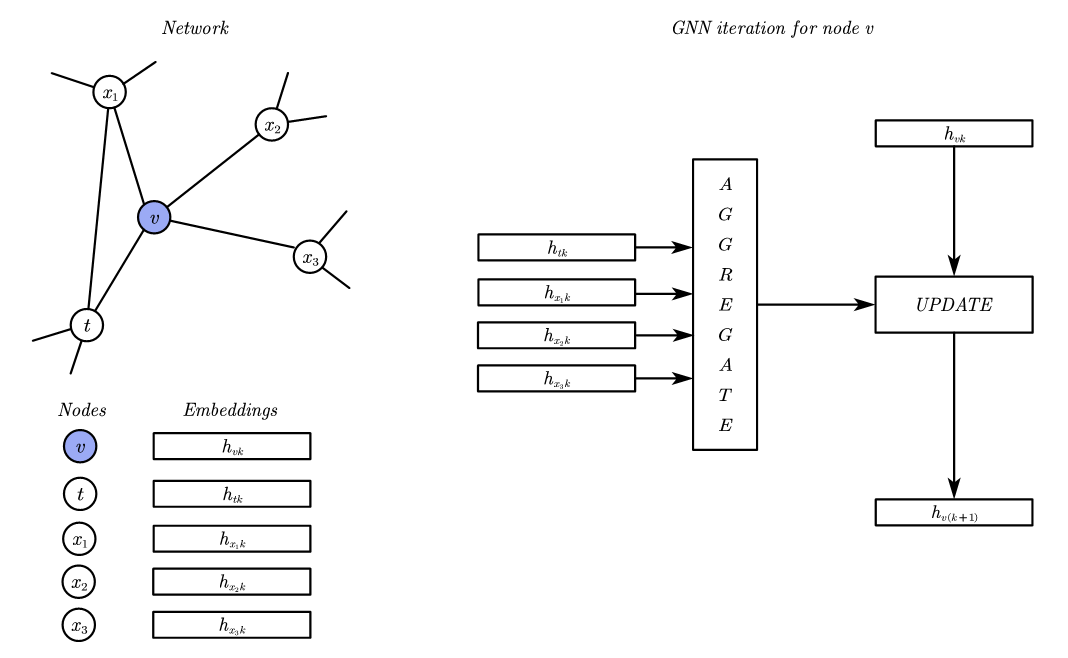
\includegraphics[width=6cm]{./figs/gnn.png}
	\caption{Iteration process of GNN}
	\label{gnn}
\end{figure}
where $h_u^{(k)}$ means the embedding vector of node u in k-th layer's output. $W^{(k)}$ and $b^{(k)}$ are k-th layer's trainable weights and bias respectively. When conducting backpropagation, these parameters will be updated based on the gradients to loss function. $\sigma$ is non-linear activation fuction, such as ReLU or Sigmoid. Following this iteration process, each GNN layer takes the last layer’s output embedding as its input, and use aggregation and update process to output a new embedding using neighborhood information. So the graph structure information will be implicitly learned in the final output. And then this output will be used to calculate loss together with ground truth label, and update GNN's parameters just as what the common deep neural networks do.

GCN is one of the most popular GNN instances, and its aggregation and update process can be expressed as the following formula. Comparing to basic GNN, GCN applies a normalization factor to each input embedding vector based on its neighborhood information.
$$h_u^{(k)}=\sigma (W^{(k)}\sum_{v\in N(u)\cup u}\frac{h_v^{(k-1)}}{\sqrt{|N(u)||N(v)|}})$$ 

GCN has shown its great ability to capture graph information and deal with graph-related tasks. Nonetheless, like other GNN, GCN is as well a iteration process of embedding vector, so the problem is that where does the intial embedding vector come from? There are three methods to generate intial embedding vector:

\textbf{one-hot vector representation} One-hot vector is widely used in deep learning area. Hence, we can allocate each node a one-hot vector for representation. However, the drawback is obvious. The total number of nodes in a gragh are usually very large, which means applying one-hot vector for each node will cause the input tensor too sparse. It's a waste of memory space and also exists negative impact on training process.

\textbf{transfer pretrained embedding} Another idea is to transfer pretrained embedding vectors from other similar tasks. It has been commonly taken advantage in Natural Language Processing area. For instance, Google's well-designed word2vec model \cite{word2vec} has generated credible embedding vectors for a large number of words. When we apply GNN to a NLP-related task, we can transfer these pretrained embedding vectors as GNN's initial embedding vectors. This method is often quite effective, but the problem is that, we cannot always have such luck to find a similar task to our graph which have been conducted before. When we apply GNN to a brand new task, this method loses its efficacy.

\textbf{trainable embbeding layer} Most deep learning frameworks provide an embedding layer. We could allocate each node a trainable stochastic embedding layer by applying the embedding layer. However, the disadvantage is that randomly initialized embedding vectors could have negative influence on training process.

Therefore, we propose a new method to combine GCN and node2vec to solve this problem. The idea is simple---use node2vec to generate embedding vectors for each node, and then apply these vectors as intial embedding vectors in GCN model. Due to the fact that the embedding vectors generated by node2vec are full of graph information, we can expect GCN can perform better with these embedding vectors as initial embedding. In the next section, we will prove our thoughts empirically via expriements. 

\section{Data}\label{sec-data}
% what datasets did you use, what types of networks do they represent, where did you obtain the data? did you do any processing? give a table describing data characteristics, such as number of nodes, edges, average degree, etc.
We evaluate baselines and our proposed model on five open source data sets. Three data sets, i.e. AIFB, MUTAG, and PubMed, are used in node classification task. Meanwhile, the goal of FB15K-237 and WordNet18RR data is link prediction. We apply built-in preprocessing APIs in Pytorch Geometric to convert the raw data into the desired format. The following is an overview of data sets.\par
\vspace{0.2cm}
\noindent\textbf{AIFB}. AIFB is a directed network modelling relationships among staff, research groups, and publications in AIFB research institute. The data set is firstly published for mining knowledge about instances with machine learning \cite{aifb}. AFIB network has 8,285 nodes, 58,086 edges, and 4 node classes. The original data can be downloaded from \url{https://data.dgl.ai/dataset/aifb.tgz}.\par
\vspace{0.2cm}
\noindent\textbf{MUTAG}. MUTAG is a benchmark dataset for node classification task. It contains a collection of chemical compounds. We use the version provided by Deep Graph Library. It is a directed network with 23,644 nodes, 148,454 edges, and 2 node classes. The download link is \url{https://data.dgl.ai/dataset/mutag.tgz}.\par
\vspace{0.2cm}
\noindent\textbf{PubMed}. PubMed is a directed citation network in biomedical field provided by paper \cite{pubmed}. In the network, nodes represent documents, while edges denote citation links. It contains 19,717 nodes, 88,648 edges, and 3 node classes. The original data is on \url{https://github.com/kimiyoung/planetoid/tree/master/data}.\par
\vspace{0.2cm}
\noindent\textbf{FB15K-237}. FB15K-237 contains knowledge relationships sourced from the Freebase database. It is a modified version of FB15K dataset. FB15K-237 network is directed, including 14,541 nodes and 544,230 edges. The link of the original data is \url{https://github.com/MichSchli/RelationPrediction/tree/master/data/FB-Toutanova}.\par
\vspace{0.2cm}
\noindent\textbf{WordNet18RR}. WordNet18RR is an improved version of WordNet18 dataset, which is a large lexical database of English. The network is directed. It contains 40,943 nodes and 93,003 edges. The original data can be found on \url{https://github.com/villmow/datasets_knowledge_embedding/tree/master/WN18RR/original}.\par
\vspace{0.2cm}
Table \ref{tab:5-data} summarizes the data sets used in our experiments.

\begin{table}[!ht]
    \centering
    \caption{Summary of Data Sets}
    \label{tab:5-data}
    \begin{tabular}{llll}
        \toprule
        \textbf{Data} & \textbf{Nodes} & \textbf{Edges} & \textbf{Classes} \\
        \midrule
        AIFB & 8,285 & 58,086 & 4\\
        MUTAG & 23,644 & 148,454 & 2\\
        PubMed & 19,717 & 88,648 & 3\\
        FB15K-237 & 14,541 & 544,230 & -\\
        WordNet18RR & 40,943 & 93,003 & -\\
        \bottomrule
    \end{tabular}
\end{table}

\section{Experiments}

% subsections on for example the experimental setup (which software, hardware and parameters did you choose), as well as the results of applying your approach to the data you described in preceding sections, leading to results that answer your research questions. you likely present some tables and figures

\subsection{Experimental Setup}
We select accuracy, recall, and macro F1 score as metrics to comprehensively assess the model performance in node classification task, while the original node2vec paper \cite{node2vec} only reports the macro F1 scores. In link prediction task, we use area under the ROC curve (AUC) as metrics, which is consistent with the node2vec paper. We compare our proposed method with two benchmarks. One is the combination of node2vec and logistic regression in \cite{node2vec}. To be specific, logistic regression model is fitted on the output features of node2vec and predict the label -- the class in node classification and the existence of the edge in link prediction. The other is GCN model \cite{gcn}. All models are implemented with scikit-learn, PyTorch, and PyTorch Geometric packages in Python. Besides, hyperparameters in models are optimized by grid search technique. We automate and parallelize the hyperparameter tuning process with Ray Tune package. Table \ref{tab:6-software} summaraizes the software environment of our experiments.

\begin{table}[!ht]
    \centering
    \caption{Summary of Software Environment}
    \label{tab:6-software}
    \begin{tabular}{lll}
        \toprule
        \textbf{Item} & \textbf{Version} & \textbf{Function}\\
        \midrule
        Python & 3.9 & Programming language.\\
        scikit-learn & 1.1.2 & Logistic regression.\\
        PyTorch & 1.12.0 & Deep learning framework.\\
        PyTorch Geometric & 2.1.0 & node2vec, GCN.\\
        Ray Tune & 2.1.0 & Hyperparameter tuning.\\
        \bottomrule
    \end{tabular}
\end{table}

As mentioned in Section \ref{sec-data}, we use default pipelines to preprocess datasets. However, there is no negative samples in data for link prediction task. To avoid the adverse impact of data imbalance, we begin with recording all nonexistent edges in a list and then randomly sample edges from the list. We set the ratio of positive samples to negative samples as 1 to 1 in experiments. The random seed in all operations related to randomness is a fixed number to ensure reproducibility. We deploy our experiments on two servers. Table \ref{tab:6-hardware} summarizes our hardware environments.

\begin{table}[!ht]
    \centering
    \caption{Summary of Hardware Environment}
    \label{tab:6-hardware}
    \begin{tabular}{llll}
        \toprule
        \textbf{Item} & \textbf{CPU} & \textbf{GPU} & \textbf{RAM}\\
        \midrule
        Server 1 & Intel Xeon Platinum 8358P & RTX A5000 & 80 GB\\
        Server 2 & Intel Xeon E5-2680 & TITAN Xp & 16 GB\\
        \bottomrule
    \end{tabular}
\end{table}

\subsection{Results: Node Classification}
Table \ref{tab:6-nc} reports the results of our experiments on node classification task. And Table \ref{tab:6-nc-hyper} lists the main hyperparameter settings. Our proposed model directly uses the best node2vec setiings to obtain the input embeddings for GCN.

\begin{table}[!ht]
    \centering
    \caption{Summary of Results in Node Classification Task}
    \label{tab:6-nc}
    \begin{tabular}{lllll}
        \toprule
        \textbf{Dataset} & \textbf{Algorithm} & \textbf{Accuracy} & \textbf{Recall} & \textbf{Macro F1}\\
        \midrule
        AIFB & node2vec & 0.9444 & 0.8750 & 0.9116\\
             & GCN & 0.9444 & 0.9375 & \textbf{0.9508}\\
             & Proposed & \textbf{0.9722} & \textbf{0.9583} & 0.9416\\
        MUTAG & node2vec & \textbf{0.7941} & 0.5652 & 0.6500\\
              & GCN & 0.7353 & 0.6193 & 0.6151\\
              & Proposed & 0.6912 & \textbf{0.7242} & \textbf{0.6857}\\
        PubMed & node2vec & 0.6650 & 0.6434 & 0.6438\\
               & GCN & 0.6770 & 0.6443 & 0.6482\\
               & Proposed & \textbf{0.6920} & \textbf{0.6508} & \textbf{0.6616}\\
        \bottomrule
    \end{tabular}
\end{table}

\begin{table}[!ht]
    \centering
    \caption{Hyperparameter Settings of Node Classification}
    \label{tab:6-nc-hyper}
    \begin{tabular}{lllll}
        \toprule
        \textbf{Algorithm} & \textbf{Parameter} & &\textbf{Value}&\\
                           &              & AIFB & MUTAG & PubMed\\
        \midrule
        node2vec & p & 0.25 & 2 & 4\\
                 & q & 0.25 & 4 & 4\\
                 & walk length & 30 & 30 & 20\\
                 & learning rate & 0.1 & 0.01 & 0.01\\
                 & embedding dims & 128 & 128 & 128\\
        GCN & \#layers & 2 & 3 & 3\\
            & learning rate & 0.01 & 0.01 & 0.05\\
            & epochs & 50 & 50 & 50\\
        Proposed & \#layers & 2 & 3 & 3\\
            & learning rate & 0.01 & 0.01 & 0.1\\
            & epochs & 50 & 50 & 50\\
       \bottomrule
    \end{tabular}
\end{table}

According to Table \ref{tab:6-nc}, the overall performance of our proposed model is better than the node2vec alone or the GCN alone. On AIFB dataset, our proposed method achieves the higher accuracy and recall than benchmarks but performs slightly worse than GCN on macro F1 score. We conjecture two main factors contribute to the gap between GCN and our proposed model on macro F1 score. The first is the relative small size of AIFB data, and the second is the randomness in model training. Results of MUTAG is a little bit interesting. Our proposed method significantly improves the performance on recall and maro F1 score, compared to the original GCN. However, the accuracy of node2vec is about 10\% higher than the proposed model. The high accuracy with the low recall of node2vec may indicate that the imbalance in data affects the training and evaluation processes. By contrast, predictions of the proposed model don't have a significant bias towards a specific class. On PubMed data, our proposed model outperforms other two baselines on all metrics, which supports the effectiveness of the proposed method.

Hyperparameter settings vary greatly from dataset to dataset. During the hyperparameter tuning process, we find that the selection of p and q is critical to node2vec, while the number of layers and the learning rate are important parameters in GCN for node classification task.

We also visualize the loss values of both GCN and our proposed method during the training. Figure \ref{fig:loss} shows the visualization results on three datasets. The integration of pretrained embeddings accelerates the convergence rate of GCN, which is consistent with our assumption.

\begin{figure}[!ht]
    \centering
    \begin{subfigure}{0.45\textwidth}
        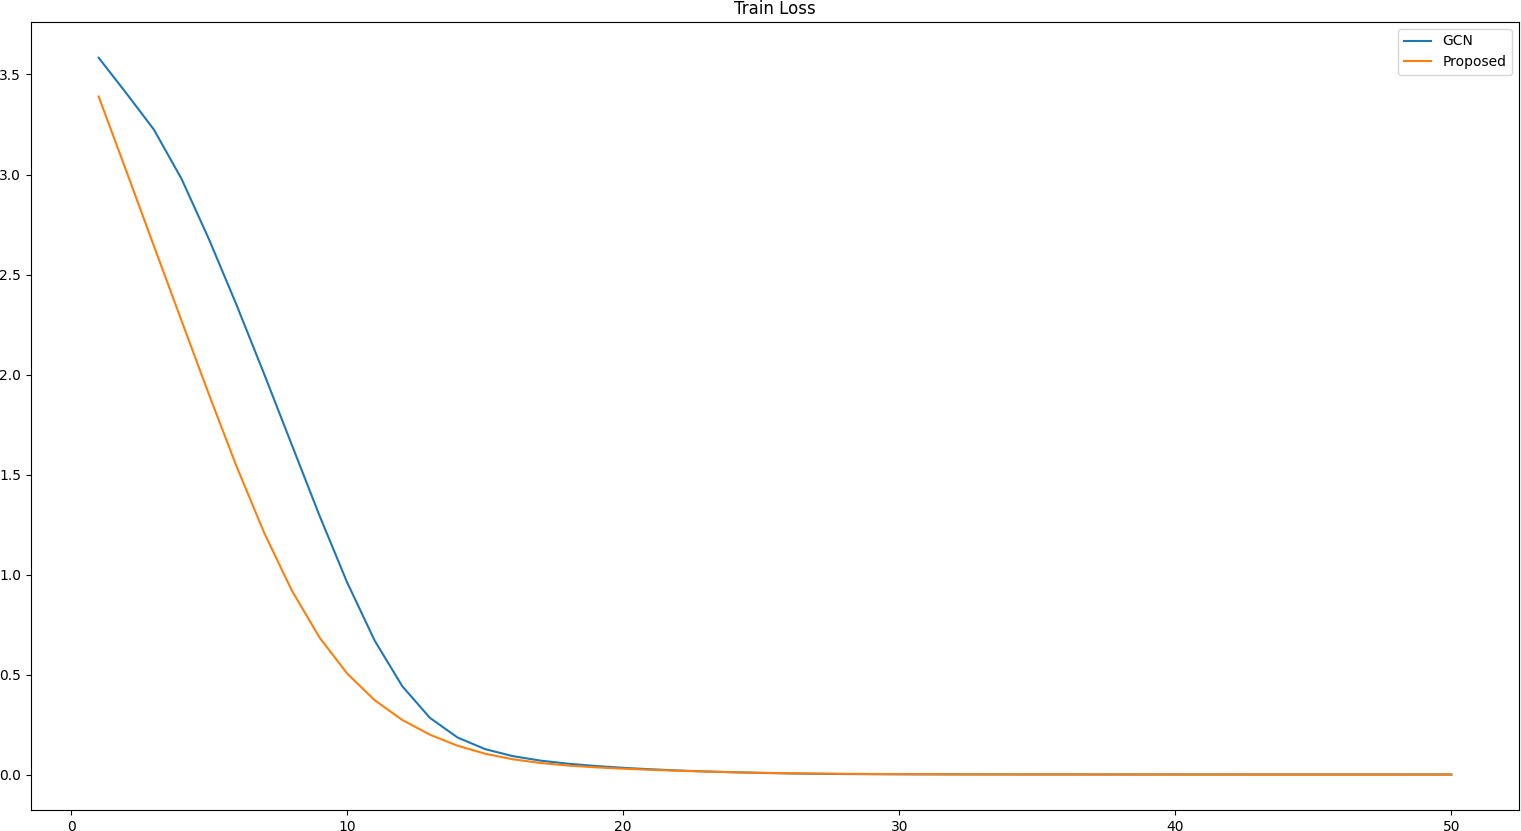
\includegraphics[width=\textwidth]{./figs/aifb-loss-2.png}
        \caption{AIFB: Training Loss}
    \end{subfigure}
    \begin{subfigure}{0.45\textwidth}
        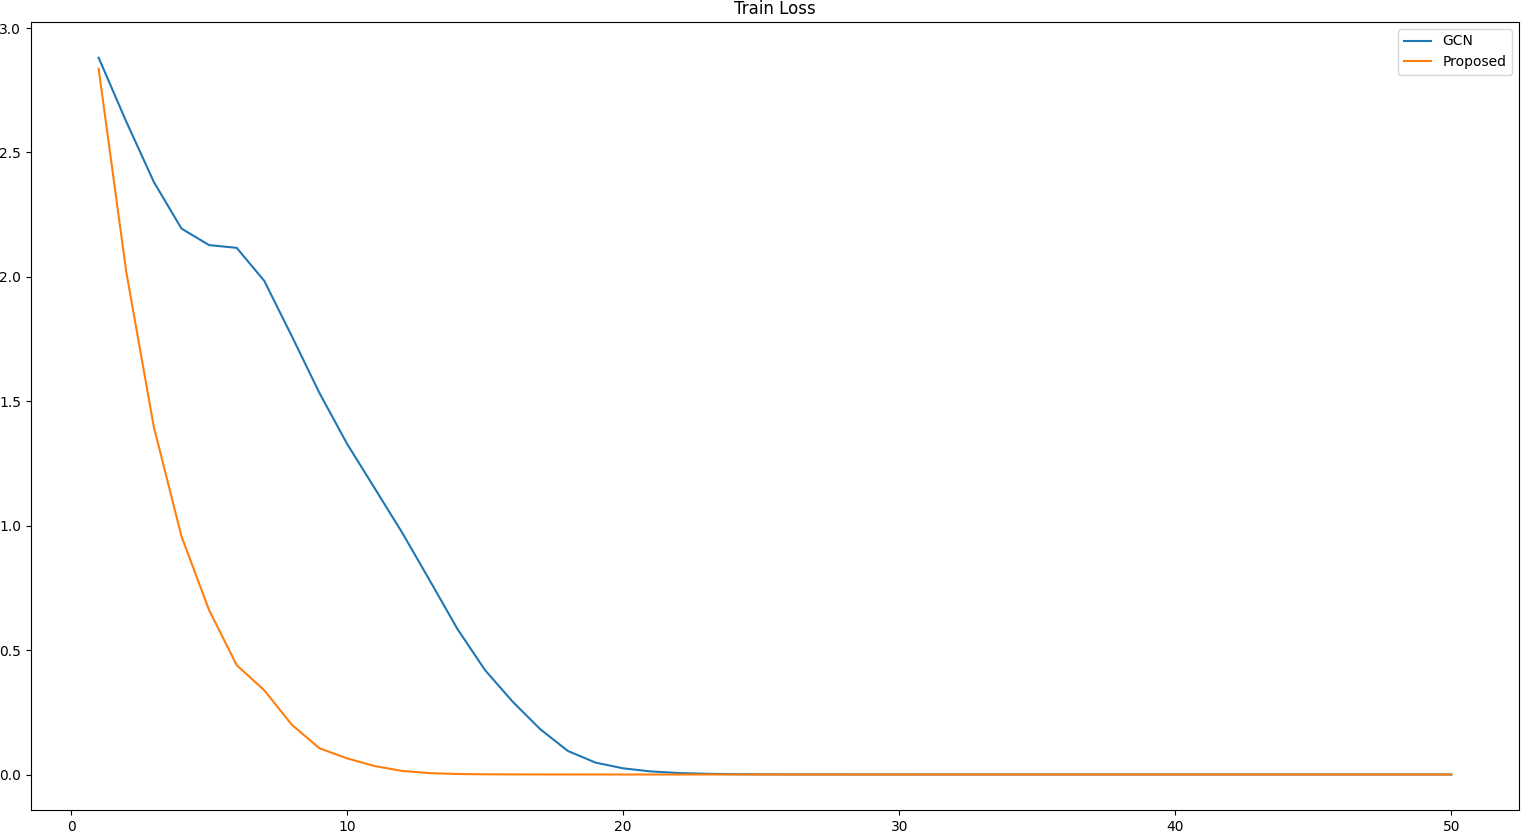
\includegraphics[width=\textwidth]{./figs/mutag-loss-2.png}
        \caption{MUTAG: Training Loss}
    \end{subfigure}
    \begin{subfigure}{0.45\textwidth}
        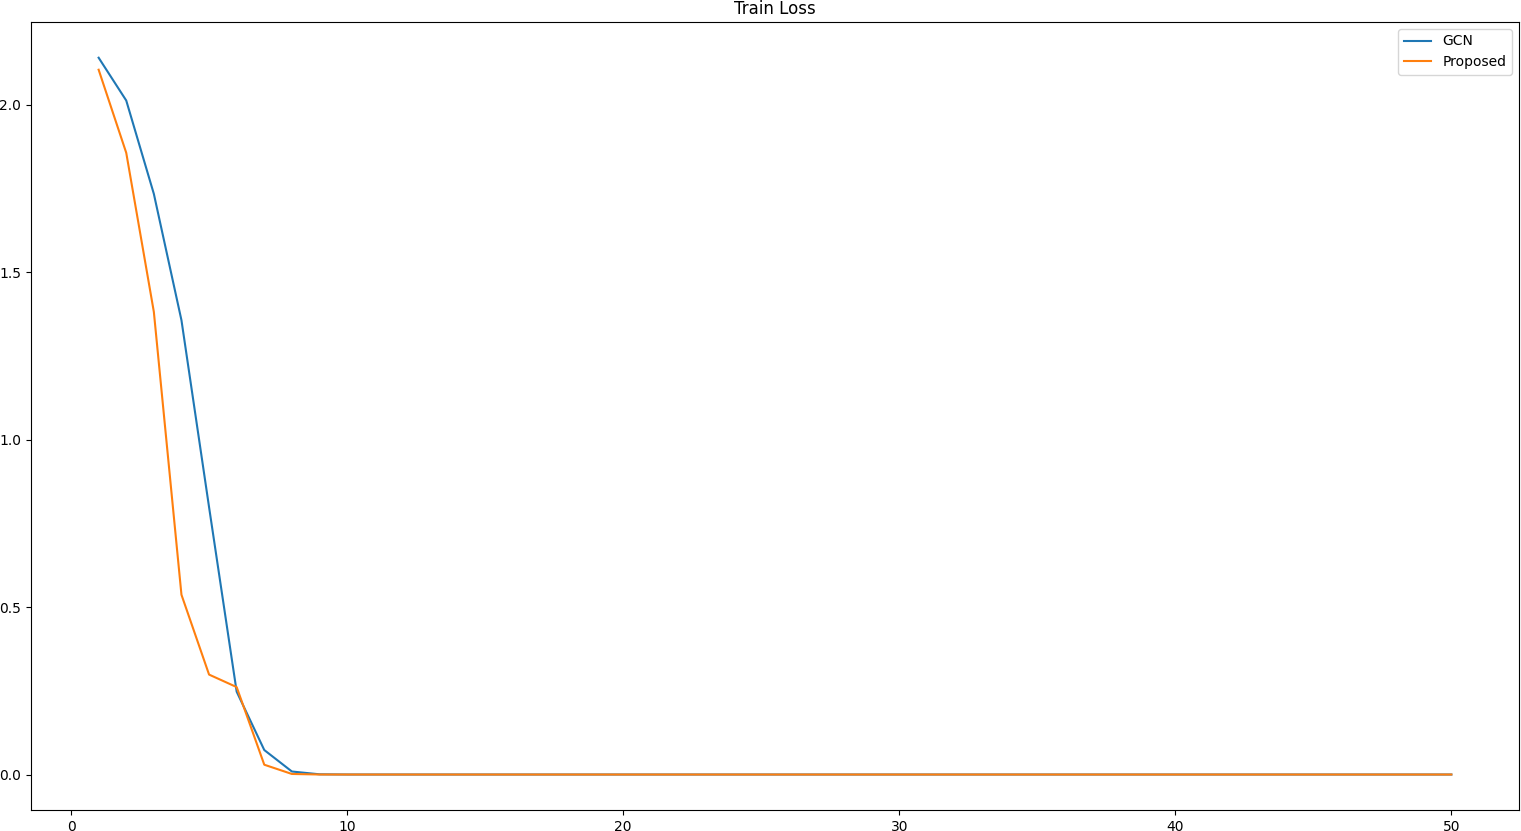
\includegraphics[width=\textwidth]{./figs/pubmed-loss-2.png}
        \caption{PubMed: Training Loss}
    \end{subfigure}
    \caption{Visualization of Training Loss}
    \label{fig:loss}
\end{figure}

\subsection{Results: Link Prediction}
We perform all four types of binary operators mentioned in Table \ref{linkop} on FB15K-237 and WordNet18RR data. Table \ref{tab:lp} reports the results of link prediction. And Table \ref{tab:lp-hyper}, \ref{tab:lp-hyper-2} summarize the hyperparameter settings used in two datasets respectively. It is worth noting that GCN link embeddings are generated by dot product operation according to the definition. Therefore, only the node2vec model and our proposed model can apply four binary operations, for they are concerned with utilizing node2vec link embeddings. We use the best node2vec settings to generate the pretrained link embeddings for the proposed model.

\begin{table}[!ht]
    \centering
    \caption{Summary of AUC in Link Prediction Task}
    \label{tab:lp}
    \begin{tabular}{llll}
        \toprule
        \textbf{Algorithm} & \textbf{Operation} & &\textbf{Dataset} \\
                      & & FB15K-237 & WordNet18RR\\
        \midrule
        node2vec & Average & 0.7875 & 0.8567\\
                 & Hadamard & 0.8626 & 0.8327\\
                 & Weighted-L1 & 0.8304 & 0.8454\\
                 & Weighted-L2 & 0.8276 & 0.8641\\
        GCN & - & 0.9816 & 0.8844\\
        Proposed & Average & 0.9810 & 0.8929\\
                 & Hadamard & \textbf{0.9819} & 0.8897\\
                 & Weighted-L1 & 0.9817 & 0.8911\\
                 & Weighted-L2 & 0.9808 & \textbf{0.8971}\\
        \bottomrule
    \end{tabular}
\end{table}

\begin{table}[!ht]
    \centering
    \caption{FB15K-237: Hyperparameter Settings}
    \label{tab:lp-hyper}
    \begin{tabular}{llll}
        \toprule
        \textbf{Algorithm} & \textbf{Parameter} & \textbf{Operation}& \textbf{Value}\\
        \midrule
        node2vec & p & Average & 2\\
                 & & Hadamard & 2\\
                 & & Weighted-L1 & 2\\
                 & & Weighted-L2 & 2\\
                 & q & Average & 0.5\\
                 & & Hadamard & 0.5\\
                 & & Weighted-L1 & 0.5\\
                 & & Weighted-L2 & 0.5\\
                 & walk length & Average & 30\\
                 & & Hadamard & 20\\
                 & & Weighted-L1 & 10\\
                 & & Weighted-L2 & 10\\
                 & learning rate & Average & 0.01\\
                 & & Hadamard & 0.01\\
                 & & Weighted-L1 & 0.1\\
                 & & Weighted-L2 & 0.1\\
                 & embedding dims & Average & 128\\
                 & & Hadamard & 64\\
                 & & Weighted-L1 & 128\\
                 & & Weighted-L2 & 128\\
        GCN & \#layers & - & 1\\
            & learning rate & - & 0.05\\
            & epochs & - & 50\\
        Proposed & \#layers & - & 1\\
                 & learning rate & - & 0.05\\
                 & epochs & - & 50\\
       \bottomrule
    \end{tabular}
\end{table}

\begin{table}[!ht]
    \centering
    \caption{WordNet18RR: Hyperparameter Settings}
    \label{tab:lp-hyper-2}
    \begin{tabular}{llll}
        \toprule
        \textbf{Algorithm} & \textbf{Parameter} & \textbf{Operation}& \textbf{Value}\\
        \midrule
        node2vec & p & Average & 2\\
                 & & Hadamard & 4\\
                 & & Weighted-L1 & 0.25\\
                 & & Weighted-L2 & 2\\
                 & q & Average & 0.25\\
                 & & Hadamard & 2\\
                 & & Weighted-L1 & 0.5\\
                 & & Weighted-L2 & 1\\
                 & walk length & Average & 20\\
                 & & Hadamard & 30\\
                 & & Weighted-L1 & 10\\
                 & & Weighted-L2 & 10\\
                 & learning rate & Average & 0.1\\
                 & & Hadamard & 0.01\\
                 & & Weighted-L1 & 0.1\\
                 & & Weighted-L2 & 0.1\\
                 & embedding dims & Average & 128\\
                 & & Hadamard & 64\\
                 & & Weighted-L1 & 128\\
                 & & Weighted-L2 & 0.1\\
        GCN & \#layers & - & 1\\
            & learning rate & - & 0.005\\
            & epochs & - & 50\\
        Proposed & \#layers & - & 1\\
                 & learning rate & - & 0.005\\
                 & epochs & - & 50\\
       \bottomrule
    \end{tabular}
\end{table}

Models with the use of GCN perform much better than the node2vec alone in link prediction task. And our proposed method achieves slightly higher AUC scores than the GCN model on both datasets. According to Table \ref{tab:lp}, different binary operations to generate node2vec link embeddings have a significant impact on model performance. Both the node2vec model and our proposed model have the best performance with hadamard operation on FB15K-237 dataset, while their highest AUC scores on WordNet18RR are achieved by applying weighted-L2 operation. Recall that the original node2vec paper \cite{node2vec} reports the hadamard operation has the best AUC sorces in link prediction task. Our conclusion is that the suitable operation depends on the properties of data. 

Hyperparameter settings are not only different from dataset to dataset but also from operation to operation. Even on the same dataset, we need to optimize hyperparameters when adopting another binary operation to obtain node2vec embeddings, which prolongs the tuning process. We use the parallelization strategy to speed up hyperparameter tuning in practice.

\section{Conclusion}
In this paper, we have proposed a method to apply node2vec to generate intial embedding vectors to improve the performance of GCN model. From experimental view, our proposed model have outperformed individual node2vec and GCN model in most tasks. 

We have conducted several experiments mainly foucus on node classification and link prediction problem. Although individual node2vec and GCN model can already have a competitive performance, our model can enhance the final result in most cases. Especially for link prediction tasks, our model can stably outperform individual node2vec and GCN model in both datasets. The experiments prove that applying the embedding vectors full of graph information generated by node2vec can exactly improve GCN's performance compared to random initialization, which now is the most common method for graph neural network. Notice that our model is composed of node2vec and GCN, which neither have special requirements to the graph data and downstream task modality. Thus, our model is a general method to enhance GCN model in graph related tasks.

There are also different kinds of GNN models rather than GCN. Because our model doesn't compulsively require any specific structure of GCN, it can be applied to improve other GNN models as well. The extention to other GNN models is very directive and easy to accomplish. So the feature work could contains conducting more experiments using many kinds of GNN models and generalize our proposal.

On account of that our model is combined by node2vec and GNN, the hyperparameters of them are also introduced and combined in our model, which makes the tuning process more complicated. In our experiments, we only empirically search a good hyperparameters setting for our model. Therefore, In feature work, to quickly obtain a good model, the theoretic anaysis of the functions of these hyperparameters are highly motived.
% summarize in at most one column the main results of the paper, stating how you addressed the problem statement and how the experiments help understand whether  the approach works (or not). end with one or two short suggestions for future work. 

\begin{acks}
% optional: acknowledgments, so people or organizations you wish to thank 
\end{acks}


\bibliographystyle{ACM-Reference-Format}
\bibliography{snacspaper} % put your references in bibtex format in snacspaper.bib

%\appendix
%\section{Appendix: Hyperparameter Settings}
% Appendixes are optional for the course project. they can contain proofs, figures or tables that do not fit in the main body of the text, but are handy as background information

\end{document}
\endinput
